\subsection{Slant Incident HWP properties}

\paragraph{Description:}
All the HWP optical properties change when it is crossed with an incoming radiation away from normal incidence.
The effect is small for degrees $<$10 away from the normal incidence and increases for larger angular deviations.
This effect has never been studied in literature but since straylight, instrumental emissions and reflections in the polarimeter 
can produce off-axis radiation crossing the HWP it is important to study it.


\subsubsection{Birifringent HWP}
\paragraph{Description:}
For a biriringent HWP, how the optical properties change with the incidence angle can be studied knowing the optical properties of the 
birifringent material versus frequency and incidence angle and suitably taking into account the effect of the ARC, always present in HWPs.


\paragraph{Plan to model and/or measure:}
Numerical simulations from cristallography properties.
Fouries Trasform Spectrometers measurements with the angle of incoming light at different, 
non-normal, incident angles with respect to the HWP.


\paragraph{Uncertainty/Range:}
Since in most cases the optical properties (refraction indices, absorption angle) come from literature
the error to associate to these properties which, with high probability, refer to different samples that ours actual ones
are source of uncertaninty. Neverthelese, the major source of uncertainty is the knowledge of how these optical properties,
generally measured at room temperature, scale with cryogenic temperatures.

\paragraph{Parameterization:}
In a birifringent crystal, the extraordinary axis has the following dependance versus the incidence angle, $i$:
\begin{equation}
n(i)=((\frac{\cos{i}}{n_e(\nu))^2}+(\frac{\sin{i}}{n_o(\nu)})^2)^(-0.5);
\end{equation}
with $n_e(\nu)$ ($n_o(\nu)$) the extraordinary (ordinary) refraction index and $\nu$ the frequency.

\begin{figure}
\centering
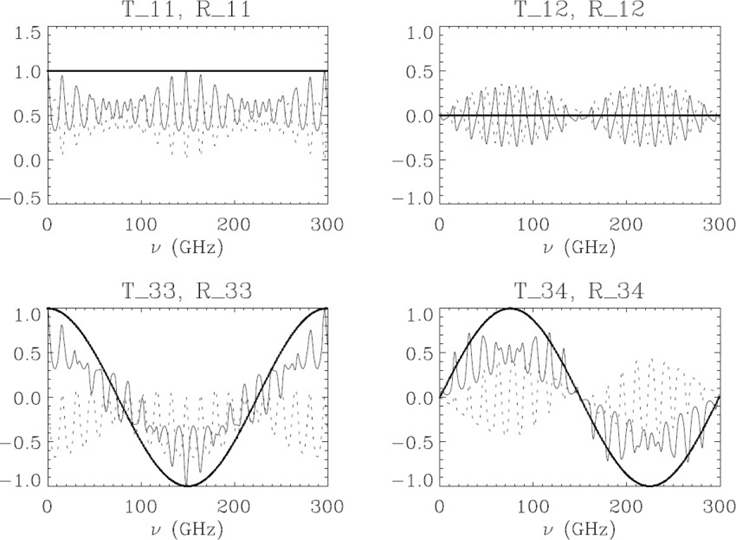
\includegraphics[width=2.5in]{figures/0deg.png}
\caption{Mueller matrix components, for both transmission (T) and reflection (R), of a real Sapphire HWP
optimized for 150 GHz (no ARC). Incoming radiation at normal incidence \cite{Salatino17}.
}\label{0deg}
\end{figure}

\begin{figure}
\centering
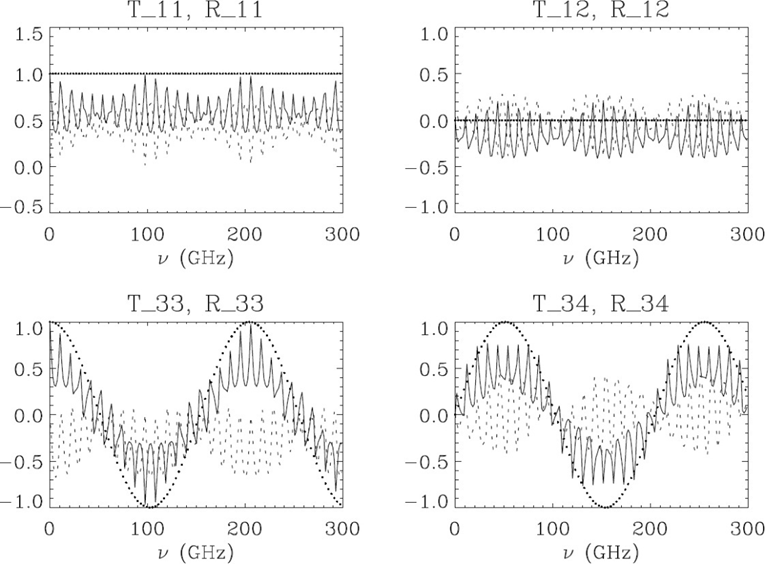
\includegraphics[width=2.5in]{figures/45deg.png}
\caption{Mueller matrix components, for both transmission (T) and reflection (R), of a real Sapphire HWP
optimized for 150 GHz (no ARC). Incoming radiation at 45deg incidence \cite{Salatino17}.}\label{45deg}
\end{figure}

%------------------------
\subsubsection{Metamaterial HWP}

\paragraph{Description:}
For a metamaterial HWP, some additional complications arise from the fact that the uderstanding of how the optical properties change with the
incident angle cannot be done analitically but require simulations with suitable softwares, such as HFSS or CST.
HFSS simulations demonstrated that the variation in the output signal increases at frequency closer to the central working frequency of the
HWP (Figs. \ref{meta1} and \ref{meta2}).

\paragraph{Plan to model and/or measure:}
Fourier Transform Spectrometers can provide experimental estimate of the optical properties. The scaling to cryogenic temperatures 
needs to assume some empirical laws.

\paragraph{Uncertainty/Range:}


\paragraph{Parameterization:}
HFSS/CST simulations with a sweep in the incident angle $i$.

\begin{figure}
\centering
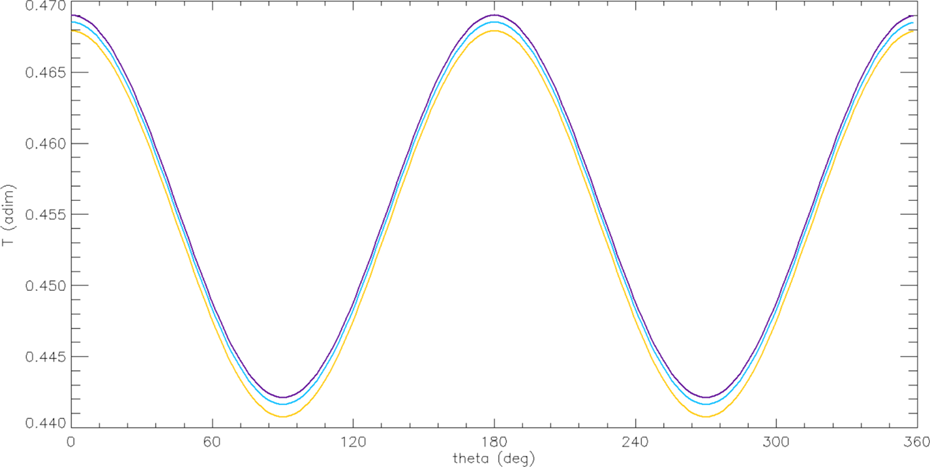
\includegraphics[width=2.5in]{figures/meta1.png}
\caption{Output signal (dimentionless units) at 70GHz from an unpolarized radiation crossing the AdvACT MF metamaterial HWP. The HWP is optimized for a frequency band centered
on 90 GHz. Violet line: -10deg, cyan line 0deg and orange 10deg incident angle. At 10deg away from the normal incidence, the output signal
changes by 0.03.}\label{meta1}
\end{figure}

\begin{figure}
\centering
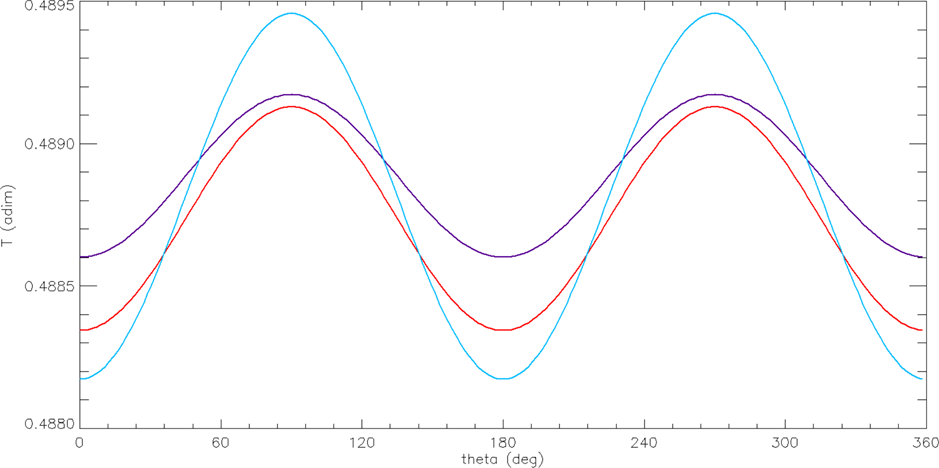
\includegraphics[width=2.5in]{figures/meta2.png}
\caption{Output signal (dimentionless units) at 90GHz from an unpolarized radiation crossing the AdvACT MF metamaterial HWP. The HWP is optimized for a frequency band centered
on 90 GHz. Violet line: -10deg, red line 0deg and cyan 10deg incident angle. At 10deg away from the normal incidence, the output signal
changes by 0.0015.}\label{meta2}
\end{figure}
